\documentclass{article}
\usepackage{enumerate}
\usepackage{amsmath}
\usepackage{amssymb}
\usepackage{graphicx}
\usepackage{subfigure}
\usepackage{geometry}
\usepackage{caption}
\usepackage{indentfirst}
\usepackage{listings}
\usepackage{xcolor} 

\usepackage{tikz}
\usetikzlibrary{circuits.ee.IEC}
\usetikzlibrary{arrows.meta}
\usetikzlibrary{calc}

\geometry{left=3.0cm,right=3.0cm,top=4.0cm,bottom=4.0cm}
\allowdisplaybreaks[4]
\title{VE311 Lab 2}
\author{Liu Yihao 515370910207}
\date{}
\lstset{
	language=Matlab, numbers=left, tabsize=4,
	framexleftmargin=1.5mm, frame=leftline,
	keywordstyle=\color{blue}\bfseries,
	identifierstyle=\bf, breaklines=true, 
	basicstyle=\normalsize,rulecolor=\color{brown}, 
	numberstyle=\color[RGB]{20,20,20}
}
\newcommand{\unit}[1]{{\rm\,#1}}

\begin{document}
\vspace*{0.25cm}

\hrulefill

\thispagestyle{empty}

\begin{center}
\begin{large}
\sc{UM--SJTU Joint Institute \vspace{0.3em} \\ Electronic Circuits \\(VE311)}
\end{large}

\hrulefill

\vspace*{5cm}
\begin{Large}
\sc{{Laboratory Report}}
\end{Large}

\vspace{2em}

\begin{large}
\sc{{Lab 2: Diodes
\vspace{0.5em}

}}
\end{large}
\end{center}

\vfill

\begin{table}[h!]
\flushleft
\begin{tabular}{lll}
Name: Chao Junyu \hspace*{2em}&
ID: 515370910206\hspace*{2em}\\
Name: Liu Yihao \hspace*{2em}&
ID: 515370910207\hspace*{2em}\\
\\

Date: 23 June 2017 

\end{tabular}
\end{table}

\hfill

\newpage
\tableofcontents
\newpage

\section{Objectives}
\begin{itemize}
	\item Test the behavior that the resistance has to temperature, humidity, high current and voltage.
	\item Understand what happened when a series of capacitors behave at different conditions.
	\item Analyze the behavior of a simple array of resistors.
\end{itemize}

\section{Experiment procedures}

\subsection{Resistor behavior}
We are going to test the behavior that the resistance has to temperature, humidity, high current and voltage. By using a resistor of 220$\unit{\Omega}$, 10$\unit{k\Omega}$ and the closest to 1$\unit{\Omega}$, perform the follow set of tests.
\begin{itemize}
	\item  
	By using a wave generator and an oscilloscope, measure the resistor response for
a voltage of 1, 5, 10 and 15 V by sweeping the frequency from 10 Hz up to 50
MHz in each case.
	\item  
	In each case heat or warm the resistance and see if there is any change in the
oscilloscope signal.
	\item
	``Carefully'' reduce the temperature of the resistance and see what happen to the
signal.
\end{itemize}

\subsection{Capacitors}
The second part considers the use of capacitors. In here, we are going to use a series of
capacitors and to understand what happened when they behave at different conditions.

\begin{itemize}
	\item
	Use the capacitors: 3.3$\unit{\mu F}$, 0.082 $\unit{\mu F}$ and 5 pF. Each one of the capacitors is to be in series with a 10 $\unit{k\Omega}$ resistor. By applying 1 $V_{pp}$ you’re going to sweep the frequency ranging from 50 MHz or the highest to 60 Hz.
	\item
	Invert the order of the devices and perform the same test.
\end{itemize}

\subsection{Inductor}
Finally, with an inductor, we are going to perform a set of experiments. By using
a simple array of a 10 kΩ resistor in series with an inductor, we’re going to analyze
the behavior of the array. By using the wave generator, we are sweeping a range of
frequencies from 50 MHz up to 1 Hz with a 1 $V_{pp}$ .

\newpage

\section{Experimental results and discussion}

\subsection{Turn on voltage}



We use the 10$\unit{k\Omega}$ resistor, which has the most apparent behavior. The voltage figure for the origin resistor was shown in Figure \ref{fig-1-1}.

%\begin{figure}[htbp]
%	\centering
%	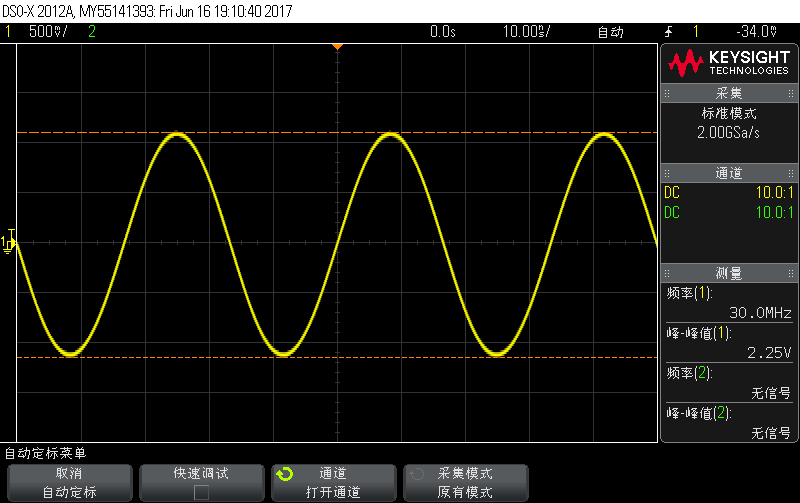
\includegraphics[width=0.7\linewidth]{imgs/scope_26.png}
%	\caption{Origin voltage figure of $R=10\unit{k\Omega}$}
%	\label{fig-1-1}
%\end{figure}

When the temperature was raised, the comparison of the origin figure and the new figure was shown in Figure \ref{fig-1-2}.

%\begin{figure}[htbp]
%	\centering
%	\subfigure[origin]{
%		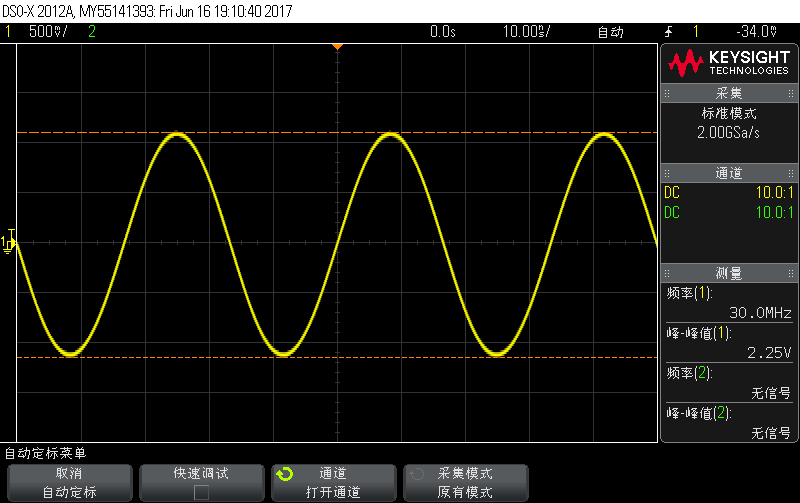
\includegraphics[width=0.45\linewidth]{imgs/scope_26.png}
%		\label{fig-1-2-1}
%	}
%	\subfigure[higher temperature]{
%		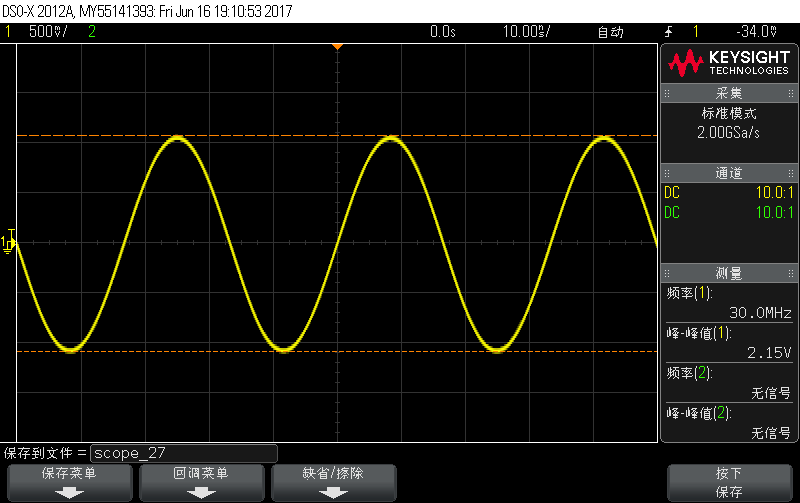
\includegraphics[width=0.45\linewidth]{imgs/scope_27.png}
%		\label{fig-1-2-2}
%	}
%	\caption{Comparison between origin figure and higher temperature}
%	\label{fig-1-2}
%\end{figure}

We can find that when the temperature rises, the voltage on the source become slightly lower, which means that the resistance becomes lower.

\newpage
When the humidity was raised, the comparison of the origin figure and the new figure was shown in Figure \ref{fig-1-3}.

%\begin{figure}[htbp]
%	\centering
%	\subfigure[origin]{
%		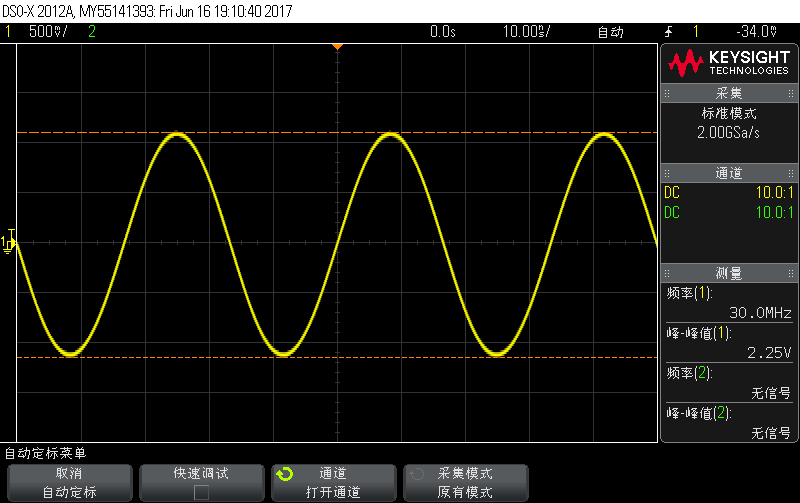
\includegraphics[width=0.45\linewidth]{imgs/scope_26.png}
%		\label{fig-1-3-1}
%	}
%	\subfigure[higher humidity]{
%		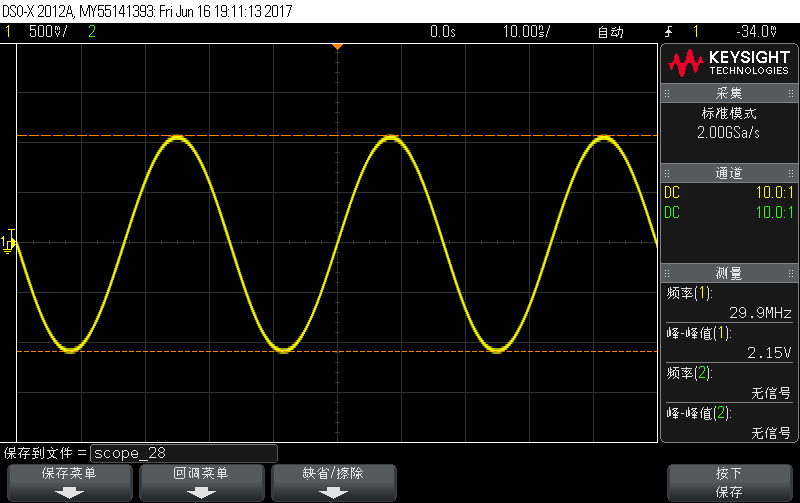
\includegraphics[width=0.45\linewidth]{imgs/scope_28.png}
%		\label{fig-1-3-2}
%	}
%	\caption{Comparison between origin figure and higher humidity}
%	\label{fig-1-3}
%\end{figure}

We can find that when the humidity rises, the voltage on the source become slightly lower, which means that the resistance becomes lower.

\newpage

\subsection{Capacitors}

We choose two capacitors, 3.3$\unit{\mu F}$ and 0.082$\unit{\mu F}$ and use the follwing circuit.

\begin{center}
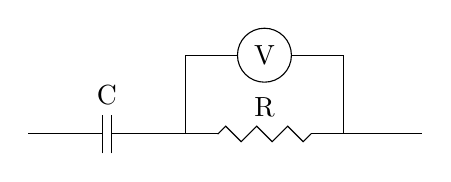
\begin{tikzpicture}[circuit ee IEC,set resistor graphic=var resistor IEC graphic]
\draw (0,0) to [resistor={info=R}] (2,0);
\draw (-2,0) to [capacitor={info=C}] (0,0);
\draw (1,1) node (V) [draw,circle] {V};
\draw (0,0) -- (0,1) -- (V) -- (2,1) -- (2,0);
\draw (2,0) -- (3,0);
\end{tikzpicture}
\end{center}

For the 3.3$\unit{\mu F}$ capacitor, the figure was shown in Figure \ref{fig-2-1}.

%\begin{figure}[htbp]
%	\centering
%	\subfigure[60 Hz]{
%		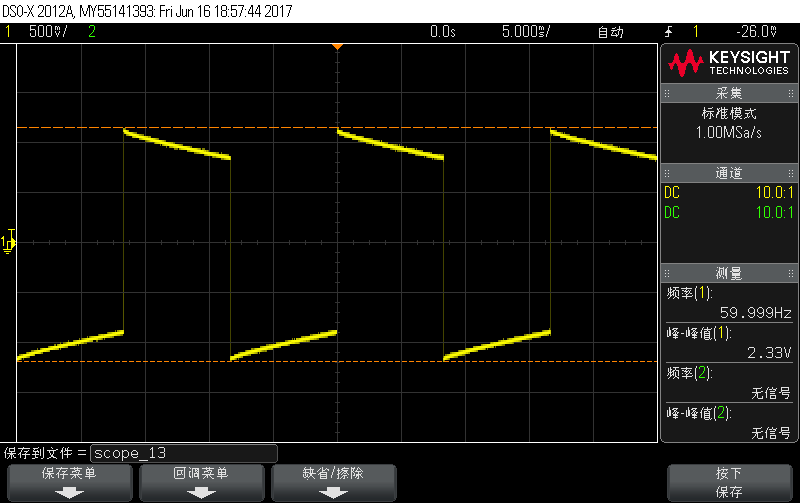
\includegraphics[width=0.45\linewidth]{imgs/scope_13.png}
%		\label{fig-2-1-1}
%	}
%	\subfigure[10 kHz]{
%		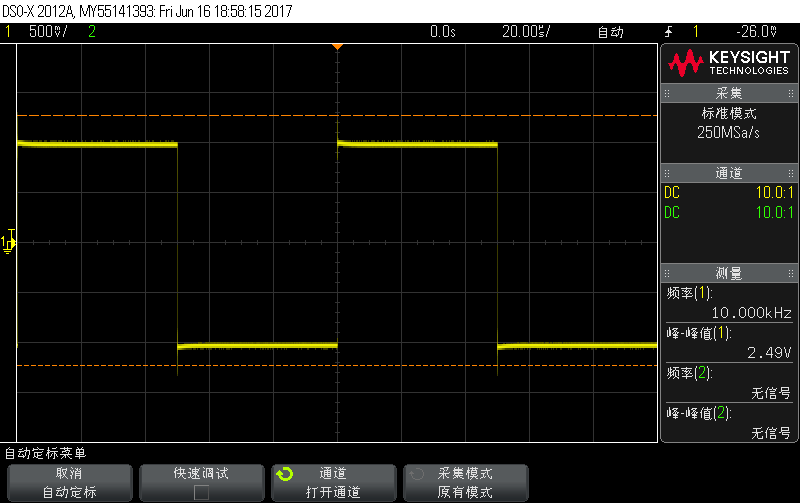
\includegraphics[width=0.45\linewidth]{imgs/scope_14.png}
%		\label{fig-2-1-2}
%	}
%	\subfigure[1 MHz]{
%		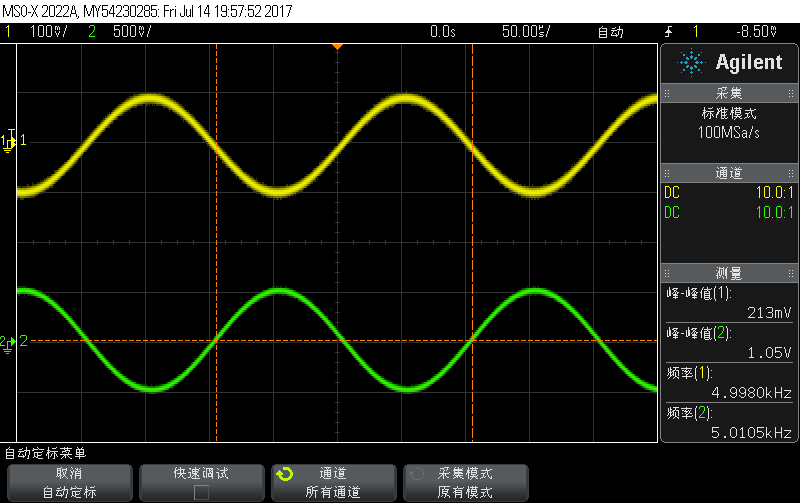
\includegraphics[width=0.45\linewidth]{imgs/scope_15.png}
%		\label{fig-2-1-3}
%	}
%	\subfigure[10 MHz]{
%		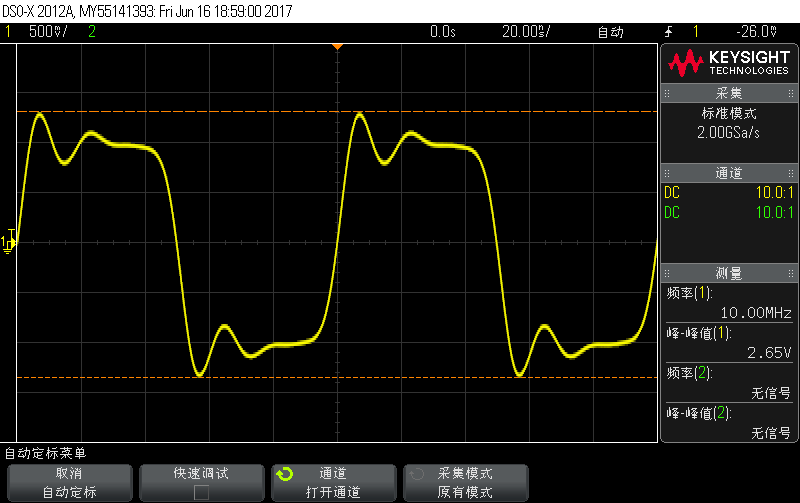
\includegraphics[width=0.45\linewidth]{imgs/scope_16.png}
%		\label{fig-2-1-4}
%	}
%	\caption{3.3$\unit{\mu F}$ capacitor}
%	\label{fig-2-1}
%\end{figure}

In an RC circuit, we have the equation
$$x(t)=K_1e^{-t/RC}+K_2$$

In Figure \ref{fig-2-1-1}, ($f=60\unit{Hz}$), $RC=10^4\unit{\Omega}\cdot3.3\unit{\mu F}=0.033\unit{k\Omega\cdot F}$, $t\in[0,\dfrac{1}{120}]\unit{s}$, so $\dfrac{t}{RC}$ is not very small, we can find some exponential curves in the figure.\\[-0.5em]

In Figure \ref{fig-2-1-2}, $t\in[0,5\times10^{-5}]\unit{s}$, $\dfrac{t}{RC}$ becomes very small, so the exponential curve converges to a straight line.\\[-0.5em]

In Figure \ref{fig-2-1-3}, $\dfrac{t}{RC}$ becomes even smaller. However, it is out of our expectation that the curve begins to behave a damping status. In theorem, it is impossible to happen according to the equation above.\\[-0.5em]

In Figure \ref{fig-2-1-4}, the curve becomes more strange, and it converges to a sine wave. \\


For the 0.082$\unit{\mu F}$ capacitor, the figure was shown in Figure \ref{fig-2-2}.

%\begin{figure}[htbp]
%	\centering
%	\subfigure[60 Hz]{
%		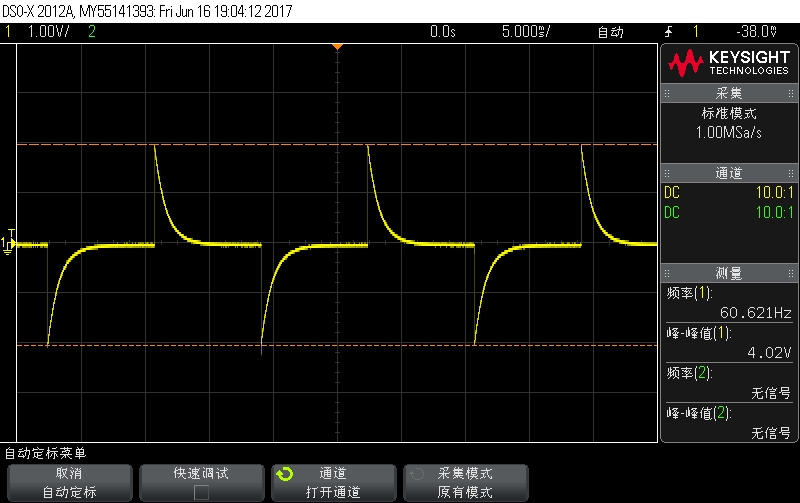
\includegraphics[width=0.45\linewidth]{imgs/scope_18.png}
%		\label{fig-2-2-1}
%	}
%	\subfigure[10 kHz]{
%		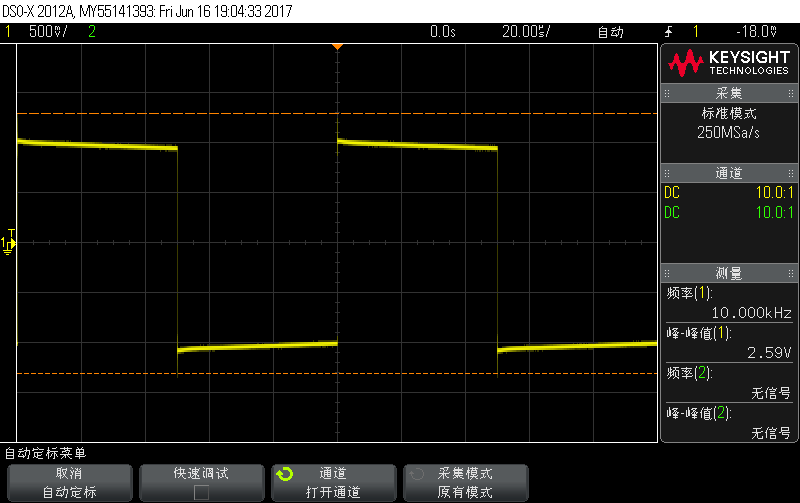
\includegraphics[width=0.45\linewidth]{imgs/scope_19.png}
%		\label{fig-2-2-2}
%	}
%	\subfigure[1 MHz]{
%		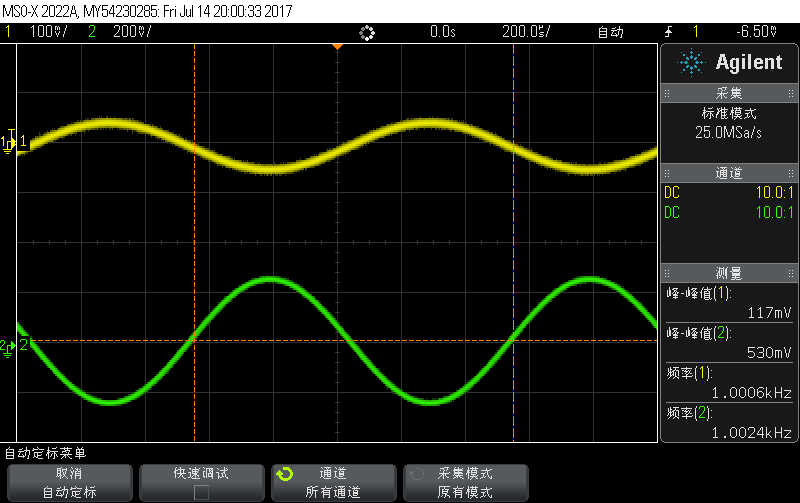
\includegraphics[width=0.45\linewidth]{imgs/scope_20.png}
%		\label{fig-2-2-3}
%	}
%	\subfigure[10 MHz]{
%		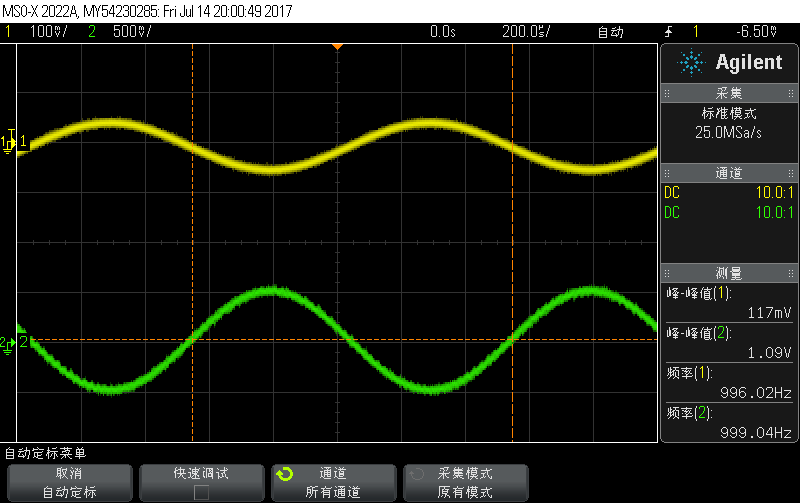
\includegraphics[width=0.45\linewidth]{imgs/scope_21.png}
%		\label{fig-2-2-4}
%	}
%	\caption{0.082$\unit{\mu F}$ capacitor}
%	\label{fig-2-2}
%\end{figure}

When the capacity of the capacitor becomes smaller, the overview of the figures doesn't change much. And in Figure \ref{fig-2-2-1}, the appearance of a more identical exponential curve is related to the increase of $\dfrac{t}{RC}$.

\newpage

\subsection{Inductor}

We use the follwing circuit.

\begin{center}
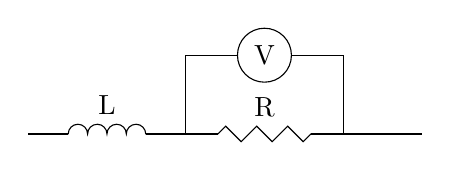
\begin{tikzpicture}[circuit ee IEC,set resistor graphic=var resistor IEC graphic]
\draw (0,0) to [resistor={info=R}] (2,0);
\draw (-2,0) to [inductor={info=L}] (0,0);
\draw (1,1) node (V) [draw,circle] {V};
\draw (0,0) -- (0,1) -- (V) -- (2,1) -- (2,0);
\draw (2,0) -- (3,0);
\end{tikzpicture}
\end{center}

%\begin{figure}[htbp]
%	\centering
%	\subfigure[10 Hz]{
%		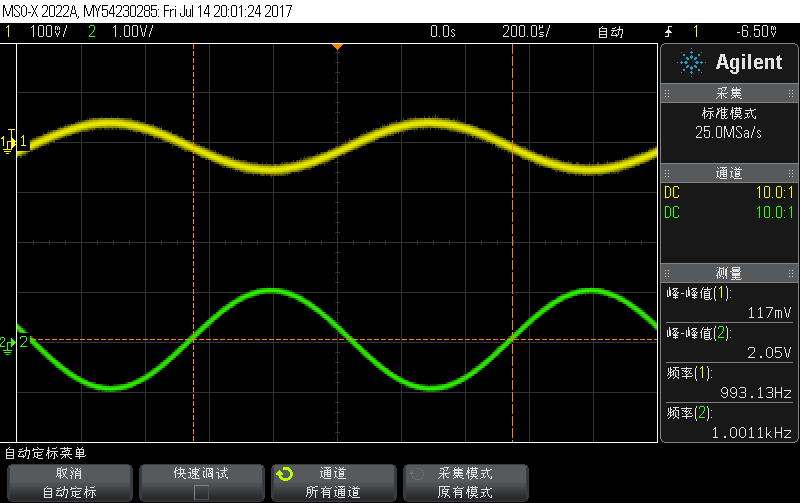
\includegraphics[width=0.45\linewidth]{imgs/scope_22.png}
%		\label{fig-3-1}
%	}
%	\subfigure[10 kHz]{
%		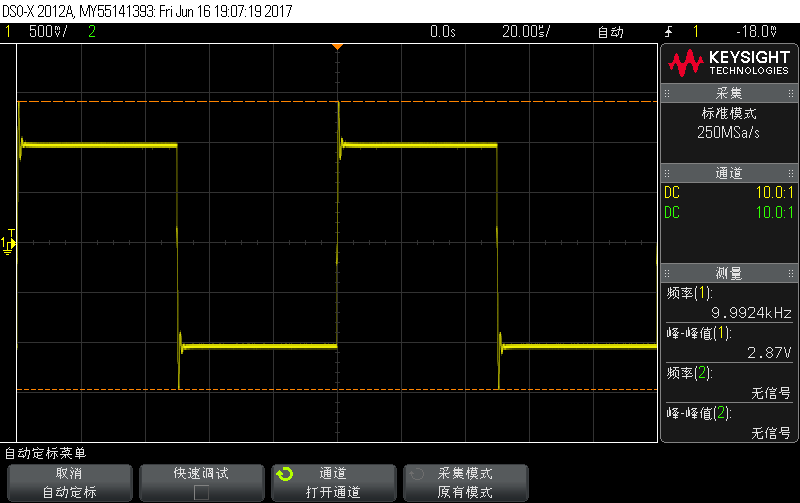
\includegraphics[width=0.45\linewidth]{imgs/scope_23.png}
%		\label{fig-3-2}
%	}
%	\subfigure[10 MHz]{
%		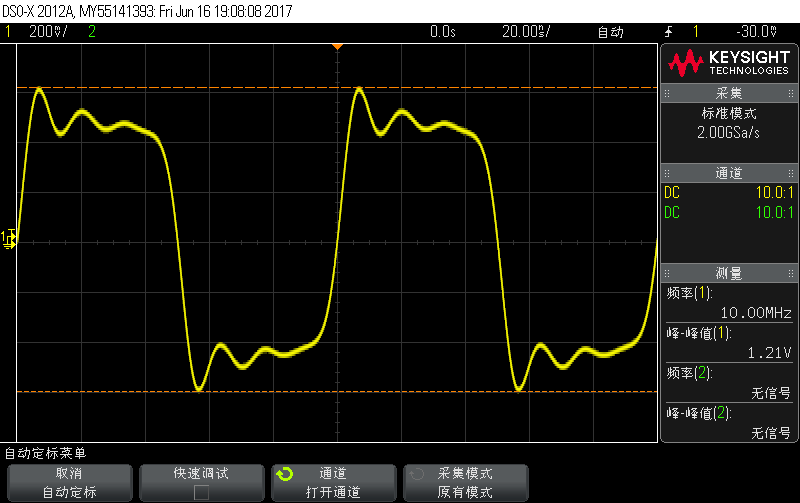
\includegraphics[width=0.45\linewidth]{imgs/scope_24.png}
%		\label{fig-3-3}
%	}
%	\subfigure[30 MHz]{
%		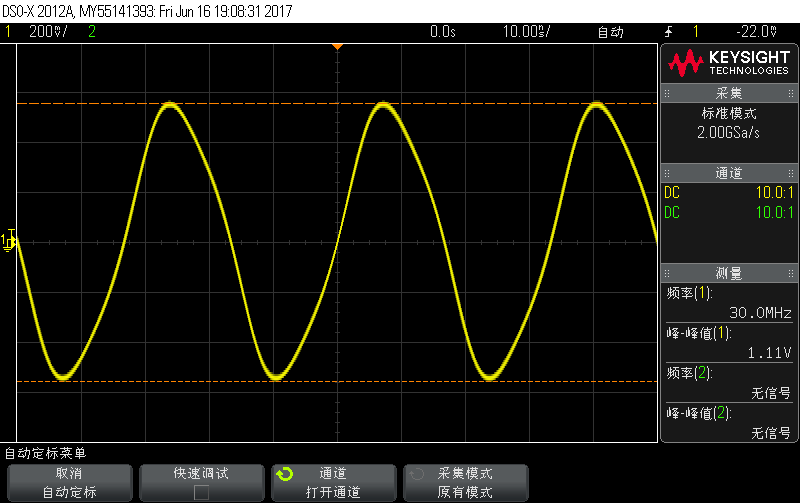
\includegraphics[width=0.45\linewidth]{imgs/scope_25.png}
%		\label{fig-3-4}
%	}
%	\caption{Inductor}
%	\label{fig-3}
%\end{figure}

In an RL circuit, we have the equation$$v(t)=K_1e^{-Rt/L}+K_2$$

Similar to the capacitors, Figure \ref{fig-3-1} and Figure \ref{fig-3-2} satisfy the equation. However, with the increasing of frequency, the figure also converges to the sine wave.

\newpage

\section{Conclusion}

In the first part, we find that when the temperature and humidity rises, the resistance of the tested resistor becomes lower. According to the physics principles, a resistor made in non-metal has such property, so we guess that the resistor is made in carbon or some other non-metal materials.\\

In the second and third part, it seems confusing to find that there is a damping, or a sine wave shown in the figure. Since the frequency is very large, the resistor in the circuit can't be identified as ideal resistor. In a non-ideal mode, a resistor can be equivalent to the following circuit.

\begin{center}
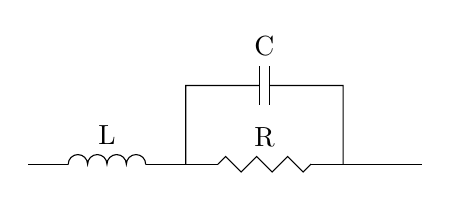
\begin{tikzpicture}[circuit ee IEC,set resistor graphic=var resistor IEC graphic]
\draw (0,0) to [resistor={info=R}] (2,0);
\draw (-2,0) to [inductor={info=L}] (0,0);
\draw (0,0) -- (0,1) to [capacitor={info=C}] (2,1) -- (2,0);
\draw (2,0) -- (3,0);
\end{tikzpicture}
\end{center}

For a typical resistor, $C\approx1\unit{pF}$, $L\approx14\unit{nH}$, when the frequency is extremely high, the circuit would become a second order RLC circuit, which have $\omega_0=\dfrac{1}{\sqrt{LC}}$, so the circuit may have a overdamped response like Figure \ref{fig-2-2-1}, or a underdamped response like Figure \ref{fig-3-4}.

\section{Reference}

\subsection{References}
\begin{enumerate}
	\item Lab2 Manual
\end{enumerate}

\end{document}
